\subsection{GCF ablation study}\label{subsec:gcf-ablation-study}
This subsection focus' on answering the following research question:
\begin{itemize}
    \item \textbf{RQ2:} How do different aggregation functions effect the performance in GCF and LightGCN?
\end{itemize}
Meng Liu et. al does not present an ablation study for BiTGCF and GCF, which LightGCN showed is important when studying the different components in NGCF \cite{lightgcn,BiTGCF}.
GCF outperformed LightGCN on all datasets used in BiTGCF \cite{BiTGCF}, and we would like understand which parts of GCF causes the increase in performance.
The GCF aggregation function is changed by either changing the layer combination to weighted summation, removing the inner product, removing self connections or only utilizing the inner product.
Examples of the changed methods can be seen in the following equations.
\textit{GCF-minus-sc} can be seen on \autoref{eq:GCF-minus-sc} where the self-connection has been removed.
On \autoref{eq:GCF-only-IP} only the inner product of the neighbour has been preserved, and is called \textit{GCF-only-IP}.
In \autoref{eq:GCF-minus-IP} the inner product has been removed and is called \textit{GCF-minus-IP}.
There are also examples where GCF utilizes summation as layer combination as used in LightGCN which can be seen on \autoref{eq:lightgcn-sum}.
The methods that use weighted summation all start with \textit{GCF-sum}.
LightGCN with concatenation as layer combination is called \textit{LightGCN-concat}.
All methods that utilize summation, would be possible to extend with ALC and BLC.
There is a possibility that GCF-sum with ALC or BLC could perform better than LightGCN with ALC or BLC.
This was however something that we decided not to pursuit and can be left as future work.
\begin{equation}
    \mathbf{e}_{u}^{(k+1)} = \sum^{}_{i \in \mathcal{N}_u}  \frac{1}{\sqrt{|\mathcal{N}_u||\mathcal{N}_i|}}\left( \mathbf{e}_i^{(k)} + \mathbf{e}_i^{(k)} \odot \mathbf{e}_u^{(k)} \right)
    \label{eq:GCF-minus-sc}
\end{equation}
\begin{equation}
    \mathbf{e}_{u}^{(k+1)} = \mathbf{e}_{u}^{(k)} + \sum^{}_{i \in \mathcal{N}_u}  \frac{1}{\sqrt{|\mathcal{N}_u||\mathcal{N}_i|}} \mathbf{e}_i^{(k)} \odot \mathbf{e}_u^{(k)}
    \label{eq:GCF-only-IP}
\end{equation}
\begin{equation}
    \mathbf{e}_{u}^{(k+1)} = \mathbf{e}_{u}^{(k)} + \sum^{}_{i \in \mathcal{N}_u}  \frac{1}{\sqrt{|\mathcal{N}_u||\mathcal{N}_i|}} \mathbf{e}_i^{(k)}
    \label{eq:GCF-minus-IP}
\end{equation}
We did not include equations for all of the methods to reduce redundancy, but the method names and descriptions are as follows:
\begin{itemize}
    \item \textbf{GCF}: The original GCF method as described in \autoref{subsubsec:GCF-embed-propagation}.
    \item \textbf{GCF-minus-sc}: GCF without self connections.
    \item \textbf{GCF-only-IP}:  GCF where $e_i^{(k)}$ has been removed in \autoref{eq:GCF-embedding}, so that GCF's graph convolutions only considers the inner product of users and items.
    \item \textbf{GCF-only-IP-minus-sc}: Implemented as GCF-only-ip but without self connections.
    \item \textbf{GCF-minus-IP}: GCF where inner product has been removed.
    \item \textbf{LightGCN-concat}: LightGCN with concatenation as layer combination.
    \item \textbf{LightGCN}: Original LightGCN as described in \autoref{subsubsec:LightGCN-embed-propagation}.
    \item \textbf{LightGCN-plus-sc}: LightGCN, but with self connections.
    \item \textbf{GCF-sum-only-IP}: Implemented as GCF-only-IP except that the layer combination method used is weighted summation.
    \item \textbf{GCF-sum}: GCF where the layer combination has been changed to weighted summation instead of concatenation.
    \item \textbf{GCF-sum-minus-sc}: Implemented as GCF-sum but without self connections.
\end{itemize}
The results can be seen on \autoref{tab:ablation-results}, where the bold results are the best performing and underlined are the second best results.
Graphs of how the performance of the methods change over epochs can be seen in \autoref{fig:GCF-NDCG-ablation-study}, \autoref{fig:GCF-NDCG-ablation-study-amazon-cell-sport} and \autoref{fig:GCF-NDCG-ablation-study-amazon-book}.
These are for the datasets yelp2020, amazon-book and amazon-cell-sport respectively.
More comprehensive figures can be seen in Appendix \ref{app:recall-results-gcf-ablation}, where the summation methods and concatenation methods are in separate figures.
\begin{table*}[]
    \centering
    \begin{tabular}{|l|l|l|l|l|l|l|l|l|}
        \hline
                             & \multicolumn{2}{c|}{Yelp2020} & \multicolumn{2}{c|}{Amazon-Cell-Sport} & \multicolumn{2}{c|}{Amazon-Book}                                                                   \\ \hline
                             & NDCG@50                       & Recall@50                              & NDCG@50                          & Recall@50           & NDCG@50             & Recall@50           \\ \hline
        GCF                  & 0.09092                       & 0.1869                                 & \underline{0.03398}              & \underline{0.06536} & 0.04032             & 0.07035             \\ \hline
        GCF-minus-sc         & 0.09084                       & 0.1879                                 & \textbf{0.03472}                 & \textbf{0.06656}    & 0.04108             & 0.07261             \\ \hline
        GCF-minus-ip         & 0.09179                       & 0.1881                                 & 0.03197                          & 0.06294             & 0.03977             & 0.06998             \\ \hline
        GCF-only-ip          & 0.07659                       & 0.1587                                 & 0.01818                          & 0.03832             & 0.03765             & 0.06607             \\ \hline
        GCF-only-ip-minus-sc & 0.08338                       & 0.1712                                 & 0.02578                          & 0.05535             & 0.03777             & 0.06621             \\ \hline
        LightGCN-concat      & 0.0856                        & 0.1735                                 & 0.03029                          & 0.05707             & 0.03798             & 0.06519             \\ \hline
        LightGCN             & \textbf{0.1064}               & \textbf{0.2106}                        & 0.033                            & 0.06278             & \underline{0.04675} & \underline{0.08129} \\ \hline
        LightGCN-plus-sc     & \underline{0.1031}            & \underline{0.2098}                     & 0.03212                          & 0.06261             & \textbf{0.04679}    & \textbf{0.08175}    \\ \hline
        GCF-sum              & 0.09724                       & 0.1988                                 & 0.03095                          & 0.06446             & 0.04075             & 0.07205             \\ \hline
        GCF-sum-minus-sc     & 0.0956                        & 0.1962                                 & 0.03075                          & 0.0629              & 0.04114             & 0.07261             \\ \hline
        GCF-sum-only-ip      & 0.09843                       & 0.199                                  & 0.02878                          & 0.06065             & 0.04114             & 0.07212             \\ \hline
    \end{tabular}
    \caption{NDCG and Recall of the changed methods.}
    \label{tab:ablation-results}
\end{table*}

\subsubsection{Concatenation and weighted summation}
Looking at Yelp2020 and Amazon-Book on \autoref{tab:ablation-results} the methods that utilize concatenation as their layer combination method generally perform worse than the methods that utilize summation.
For Yelp2020 the best performing concatenation method is \textit{GCF-minus-ip} with 0.09179 in NDCG and the best performing weighted summation is \textit{LightGCN} with 0.1064 in NDCG, which is an increase of 13.7 \%.
In Amazon-Book the best performing weighted summation method is \textit{LightGCN-plus-sc} with NDCG of 0.04679 and best concatenation method is \textit{GCF-minus-sc} with 0.04108, which is an increase 12.2 \%.
For Amazon cell sport concatenation performs better than weighted summation.
\textit{GCF-minus-sc} is the best performing concatenation method with NDCG of 0.03472 and \textit{LightGCN} is the best weighted summation method of 0.033, which is an increase of 4.9 \%.
For Yelp2020 as seen on \autoref{fig:GCF-NDCG-ablation-study} most concatenation methods learn faster than the summation methods, but the concatenation methods are also prone to early stopping because they start to decline in performance.
This is also the case for Amazon-Book on \autoref{fig:GCF-NDCG-ablation-study-amazon-book}, although some concatenation methods are not prone to early stopping.
For Amazon-Cell-Sport the methods perform differently compared to the Yelp2020 dataset as seen on \autoref{fig:GCF-NDCG-ablation-study-amazon-cell-sport}.
The summation methods train for a lower number of epochs compared to the Yelp2020 dataset.
This could be because amazon-cell-sport is a smaller dataset than Yelp2020.
Generally it can be seen that GCF and GCF-minus-sc perform better on Amazon-Cell-Sport compared to the other methods in \autoref{fig:GCF-NDCG-ablation-study-amazon-cell-sport}.
LightGCN performs better than the GCF methods that utilize weighted summation as their layer combination method.
However with Amazon-Cell-Sport the results vary less between the methods, although \textit{gcf-sum-only-ip} is clearly performing worst.
\begin{figure}[]
    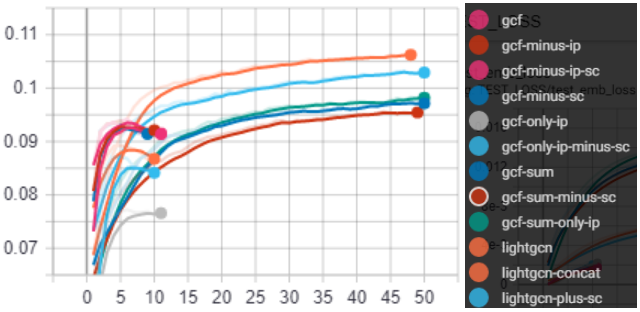
\includegraphics[width=\linewidth]{figures/gcf-all-ndcg.png}
    \caption{NDCG@50 for the Yelp2020 dataset.}
    \label{fig:GCF-NDCG-ablation-study}
\end{figure}
\begin{figure}[]
    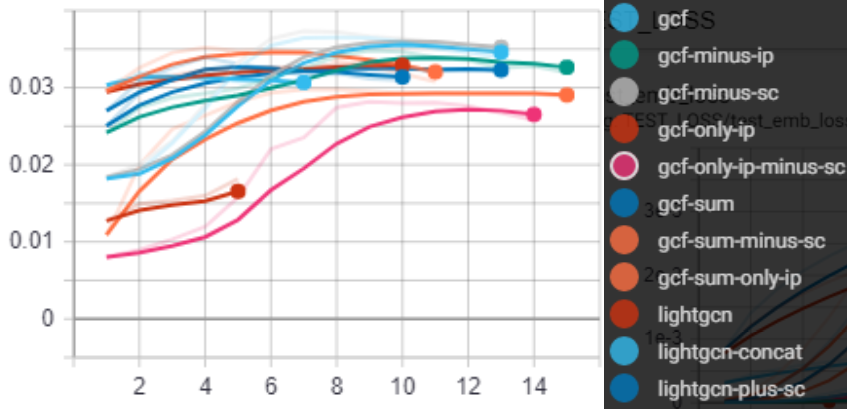
\includegraphics[width=\linewidth]{figures/amazon-cell-sport-gcf-all-ndcg.png}
    \caption{NDCG@50 for the Amazon-Sport-Cell dataset.}
    \label{fig:GCF-NDCG-ablation-study-amazon-cell-sport}
\end{figure}
\begin{figure}[]
    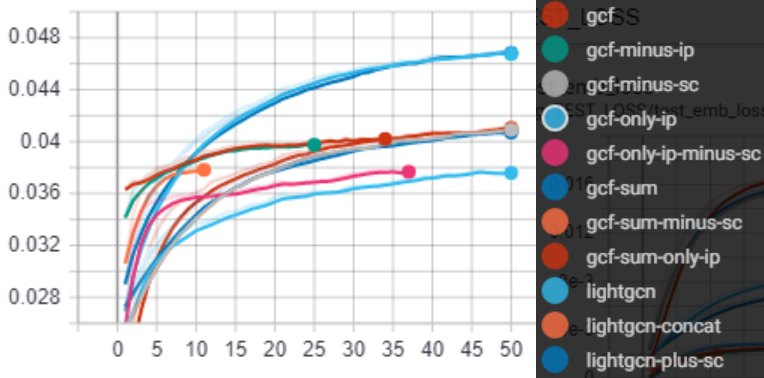
\includegraphics[width=\linewidth]{figures/amazon-book-gcf-all-ndcg.png}
    \caption{NDCG@50 for the Amazon-Book dataset.}
    \label{fig:GCF-NDCG-ablation-study-amazon-book}
\end{figure}

\subsubsection{Inner product}
Methods that use weighted summation perform worse over time when utilizing inner product.
The only exception is Recall@50 on Amazon-Cell-Sport for \textit{GCF-sum} which performs better than LightGCN.
This could also simply be because the inner product in general is beneficial for datasets where users or items have few connections.
For \textit{GCF} and \textit{GCF-minus-ip} it makes a small difference to add inner product in Yelp2020 and Amazon-Book, however for Amazon-Cell-Sport the method using inner product performs 6 \% better for NDCG@50 and 3.8 \% better for Recall@50.
These result can indicate that utilizing inner product is favorable for datasets with few connections, but can be difficult to conclude when only using three datasets.

\subsubsection{Self connections}
When comparing the counter parting methods on \autoref{tab:ablation-results} that either utilize or do not utilize self connections there is often a minimal difference on the results.
For LightGCN, GCF and GCF sum, using self connections makes a small difference.
For \textit{LightGCN} and \textit{LightGCN-plus-sc} it varies which one performs best, but \textit{GCF-minus-sc} outperforms \textit{GCF} by a small amount most of the time.
This is probably dependent on how many connections there are in the dataset.
It seems datasets with few connections declines in performance by adding self connections, and datasets with many connections benefit from adding self connections.
This would probably be because when the node has few connections, the self connection will have a large influence on the embedding.
Interestingly \textit{gcf-only-ip-minus-sc} performs significantly better than \textit{gcf-only-ip} on Yelp2020 and Amazon-Cell-Sport, which can indicate that self connections are harmful for performance, if you only use inner product in the convolutions.
However on Amazon-Book it does not make a large difference, which could be because users and items in this dataset has many interactions.

\subsubsection{Conclusion}
The best performing methods is dependent on the dataset.
\textit{GCF-minus-sc} is the best performing on Amazon-Cell-Sport, which is the smallest datasets, that also includes a lot of items with very few interactions.
\textit{LightGCN} and \textit{LightGCN-plus-sc} is performs good in all three datasets, and is still the third best performing method in Amazon-Cell-Sport.
We assume that a combination of inner product and concatenation is beneficial for learning on small datasets or datasets with few interactions between users and items.
But on the larger datasets, \textit{LightGCN} and \textit{LightGCN-plus-sc} are better performing methods.
